\chapter{Implementação do sistema}\label{cap:implementacao}

Este capítulo descreve a implementação do S.R.I. na versão consolidada do estágio. São apresentados a organização do código em camadas, o ambiente e as bibliotecas efetivamente utilizados, a evolução do esquema do banco de dados local, a implementação de cada caso de uso, o algoritmo de ordenação das paradas e as decisões adotadas para o tratamento de falhas. Ao final, são registrados os resultados da verificação por análise estática e por testes automatizados.

\section{Organização do código em camadas}

A versão inicial do aplicativo concentrava o acesso ao banco de dados em uma única classe e mantinha a lógica de negócio dentro das telas. À medida que os casos de uso de geração de rotas, de rotas salvas e de gerenciamento de usuário foram incorporados, essa organização passou a dificultar tanto a leitura do código quanto a sua verificação por testes. A versão consolidada adota, por isso, uma separação explícita em camadas, ilustrada na Figura \ref{fig:diagrama-de-camadas}.

\begin{figure}[!ht]
    \centering
    \caption{Organização do código em camadas}
    \label{fig:diagrama-de-camadas}
    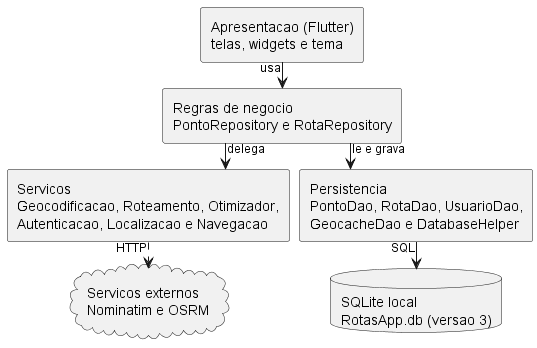
\includegraphics[width=1\linewidth]{imagens/diagrama-de-camadas.png}
    \vspace{2pt}
    \footnotesize Fonte: o próprio autor (2026)
\end{figure}

A camada de \textbf{apresentação} reúne as telas e os componentes visuais reutilizáveis. As telas não executam consultas ao banco nem chamam diretamente os serviços externos: elas solicitam operações às camadas inferiores e tratam apenas o estado da interface.

A camada de \textbf{regras de negócio} é composta pelos repositórios \texttt{PontoRepository} e \texttt{RotaRepository}. É nessa camada que residem as decisões do domínio, como reaproveitar as coordenadas já gravadas quando o endereço não foi alterado em uma edição, gravar o ponto mesmo quando a geocodificação falha e orquestrar a ordenação das paradas antes de solicitar o trajeto.

A camada de \textbf{serviços} reúne as classes com responsabilidade única e bem delimitada: a geocodificação de endereços, o cálculo de trajetos por vias, a ordenação das paradas, a autenticação, o acesso à posição do dispositivo e os cálculos da navegação assistida. Esses serviços não conhecem a interface nem gravam dados diretamente.

A camada de \textbf{persistência} contém os objetos de acesso a dados, um por conjunto de tabelas, e a classe \texttt{DatabaseHelper}, responsável exclusivamente por abrir a conexão, criar o esquema e aplicar as migrações.

A montagem das dependências é centralizada na classe \texttt{Dependencias}, que instancia os serviços e repositórios uma única vez e os entrega prontos às telas. Essa classe também é o ponto pelo qual os testes automatizados substituem o banco real por um banco em memória e o cliente HTTP real por um cliente simulado, sem que nenhuma tela precise ser alterada para isso.

\section{Ambiente e bibliotecas utilizados}

A Tabela \ref{tab:bibliotecas} relaciona as versões efetivamente utilizadas na versão consolidada, conforme registrado no arquivo de controle de dependências do projeto.

\begin{table}[!ht]
    \centering
    \caption{Bibliotecas e versões utilizadas na implementação}
    \label{tab:bibliotecas}
    \begin{tabular}{p{5cm}p{2cm}p{6cm}}
        \hline
        \textbf{Componente} & \textbf{Versão} & \textbf{Finalidade no projeto} \\
        \hline
        Flutter & 3.41.5 & Framework de interface e compilação para múltiplas plataformas \cite{flutter2024} \\
        Dart & 3.11.3 & Linguagem de programação do aplicativo \cite{dart2024} \\
        sqflite & 2.4.2 & Acesso ao banco de dados SQLite embarcado \cite{sqflite2024} \\
        flutter\_map & 8.2.2 & Renderização do mapa a partir de blocos cartográficos \cite{fluttermap2024} \\
        latlong2 & 0.9.1 & Representação de coordenadas geográficas \\
        http & 1.6.0 & Requisições aos serviços de geocodificação e de roteamento \\
        geolocator & 14.1.1 & Leitura da posição do dispositivo \cite{geolocator2024} \\
        crypto & 3.0.7 & Resumo criptográfico para a derivação da senha \\
        path & 1.9.1 & Composição do caminho do arquivo do banco de dados \\
        flutter\_lints & 5.0.0 & Regras de análise estática do código \\
        sqflite\_common\_ffi & 2.4.0+3 & Execução do SQLite nos testes automatizados \\
        \hline
    \end{tabular}
    \vspace{2pt}
    \footnotesize Fonte: o próprio autor (2026)
\end{table}

Todas as bibliotecas utilizadas são de código aberto e dispensam a contratação de licenças ou de chaves de acesso comerciais, o que atende à restrição de custo registrada na Especificação Complementar \cite{sriEspecComp2025, redhatOpenSource2024}.

\section{Evolução do esquema do banco de dados local}

O banco de dados local evoluiu em quatro versões, sempre de forma incremental e sem perda dos dados já cadastrados. A primeira versão continha apenas a tabela de pontos, correspondente ao caso de uso de gerenciamento de locais. A segunda versão acrescentou as tabelas de rotas e de itens de rota, necessárias para registrar a sequência ordenada de visitas. A terceira versão acrescentou as tabelas de usuários, de sessão e de cache de endereços, além da coluna que vincula cada ponto ao seu proprietário. A quarta versão acrescentou a tabela de preferências, que guarda a opção de manter a sessão entre execuções e a conta lembrada na tela de acesso.

A migração entre versões é aplicada pela própria classe \texttt{DatabaseHelper}, por meio do mecanismo de versionamento do SQLite. A passagem para a versão 3 utiliza a instrução de acréscimo de coluna, que preserva os registros existentes em vez de recriar a tabela. Os pontos cadastrados antes da existência de contas permanecem sem proprietário e são vinculados à primeira conta criada no dispositivo, em vez de ficarem órfãos ou inacessíveis. A passagem para a versão 4 apenas cria uma tabela nova, sem tocar nos dados existentes, de modo que a atualização é segura mesmo em um aparelho já em uso.

Duas decisões de integridade merecem registro. A primeira é a ativação explícita das chaves estrangeiras na abertura da conexão, sem a qual o SQLite aceitaria as declarações de integridade sem aplicá-las. A segunda é a gravação das rotas dentro de uma transação: como uma rota envolve a inserção em duas tabelas, a gravação atômica impede que uma falha intermediária deixe uma rota cadastrada sem os seus pontos.

\section{Implementação dos casos de uso}

\subsection{UC01: gerenciamento de locais}

O cadastro de um local solicita o nome e o endereço, converte o endereço em coordenadas por meio do serviço Nominatim e grava o registro no banco local. A tela inicial lista os pontos ordenados alfabeticamente e oferece as ações de editar, excluir e visualizar no mapa, esta última centrada nas coordenadas gravadas e com a indicação do ponto.

Duas decisões de implementação melhoram o comportamento em uso real. Na edição, quando o endereço não foi alterado, as coordenadas já gravadas são reaproveitadas e nenhuma consulta externa é realizada, o que torna a correção do nome instantânea. Além disso, se a conversão do endereço falhar, o ponto é gravado mesmo assim, sem coordenadas, e a interface informa que o endereço poderá ser localizado depois. Essa escolha preserva o cadastro em situação de conectividade instável, conforme a premissa registrada na Visão do produto \cite{sriVisao2025}.

\subsection{UC02: geração de rotas}

A montagem de uma rota ocorre em duas etapas. Na primeira, o usuário seleciona os pontos que comporão o trajeto, escolhe entre a modalidade ponto a ponto e a modalidade em circuito e, opcionalmente, define o ponto de partida e o ponto de chegada. Na segunda, o sistema apresenta o resultado do cálculo: o traçado sobre o mapa, os marcadores numerados na ordem de visita, a distância total, a duração estimada e o ganho obtido na ordenação.

A modalidade em circuito determina que o trajeto retorne ao ponto de partida, o que é obtido acrescentando-se a coordenada inicial ao final da sequência enviada ao serviço de roteamento. Qualquer alteração na seleção de pontos invalida o resultado já calculado, de modo que o usuário nunca grave uma rota diferente da que está visualizando.

A interação entre os componentes durante o cálculo é apresentada na Figura \ref{fig:sequencia-gerar-rota}. O diagrama evidencia a separação de responsabilidades entre a tela, o repositório, o serviço de ordenação, o serviço de roteamento e o objeto de acesso a dados, e mostra os dois desvios previstos: a recusa do cálculo quando a seleção é insuficiente e o recuo para a estimativa local quando o serviço de roteamento não responde. A gravação aparece como um trecho opcional, que só ocorre depois que o usuário confirma a operação, e é executada dentro de uma transação.

\begin{figure}[p]
    \centering
    \caption{Diagrama de sequência do caso de uso UC02 (geração de rotas)}
    \label{fig:sequencia-gerar-rota}
    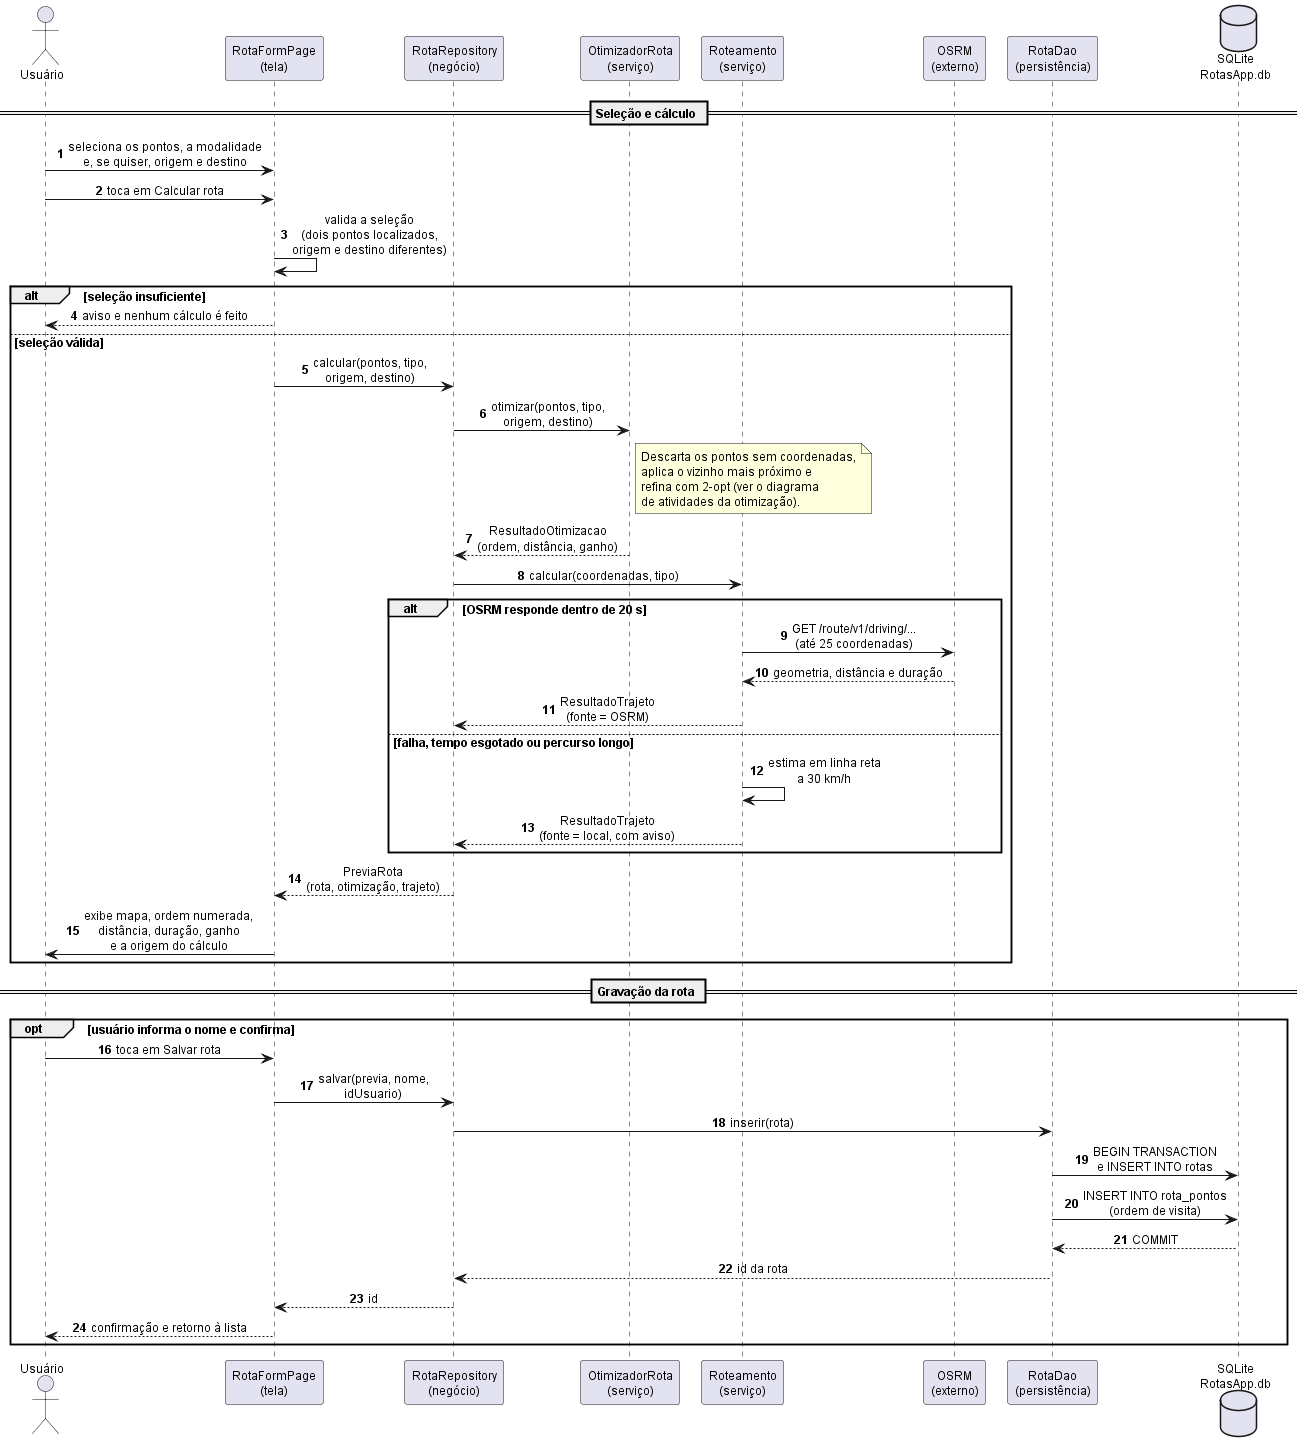
\includegraphics[width=\linewidth]{imagens/sequencia-gerar-rota.png}
    \vspace{2pt}
    \footnotesize Fonte: o próprio autor (2026)
\end{figure}

\subsection{UC03: gerenciamento de rotas salvas}

As rotas calculadas podem ser nomeadas e gravadas para reutilização. A listagem das rotas salvas apresenta o nome, a modalidade, a quantidade de paradas, a distância e a duração, e oferece as operações de consulta, de edição e de exclusão. A consulta de uma rota salva exibe novamente o traçado sobre o mapa e a ordem de visita, e é o ponto de partida para a navegação assistida.

A gravação da rota persiste a sua geometria, de modo que a reabertura de um trajeto já calculado não exige uma nova consulta ao serviço externo. A exclusão de um ponto cadastrado remove automaticamente o vínculo desse ponto com as rotas que o utilizavam, sem eliminar as rotas remanescentes.

\subsection{UC04: gerenciamento de usuário}

O acesso ao aplicativo exige autenticação prévia, conforme estabelecido na Especificação Complementar \cite{sriEspecComp2025}. A implementação compreende a criação de conta, o acesso, a manutenção dos dados cadastrais, a troca de senha e a exclusão da conta.

A senha não é armazenada em texto legível. Para cada conta é sorteado um sal aleatório de dezesseis bytes, e o valor gravado resulta da aplicação repetida do resumo criptográfico SHA-256, em dez mil iterações, sobre a composição do sal com a senha. Essa repetição, denominada alongamento de chave, encarece substancialmente a tentativa de adivinhação por força bruta. Trata-se de um esquema didático: um sistema em produção deveria empregar algoritmos projetados especificamente para senhas, como PBKDF2, bcrypt ou Argon2. A comparação entre o valor calculado e o valor gravado é feita sem interrupção na primeira diferença, de modo que o tempo de resposta não revele quantos caracteres iniciais estavam corretos.

A sessão do usuário é registrada em uma tabela de linha única, o que permite restaurar o acesso quando o aplicativo é reaberto sem manter a senha em memória. A mensagem devolvida em uma tentativa de acesso malsucedida é idêntica para e-mail inexistente e para senha incorreta, o que evita revelar quais endereços estão cadastrados no aparelho.

Como a autenticação é obrigatória, a tela de acesso foi construída para exigir o mínimo de digitação, de modo que a exigência não se transforme em atrito diário. Duas medidas atendem a esse objetivo.

A primeira é a \textbf{conta lembrada}: o e-mail e o nome do último acesso são gravados na tabela de preferências, e a tela de acesso passa a exibir um cartão de identificação da conta no lugar do campo de e-mail. O usuário digita apenas a senha, e o foco já começa nesse campo, de modo que o acesso se completa com o próprio botão de confirmação do teclado. Um botão de troca de conta permite informar outro usuário quando necessário.

A segunda é a opção \textbf{manter conectado}, marcada por padrão. Quando está marcada, a sessão é gravada no banco e o aplicativo abre direto no conteúdo nas execuções seguintes; quando não está, nenhuma sessão é gravada e a senha volta a ser pedida na próxima abertura, ainda com o e-mail lembrado. Para que esse comportamento funcione sem depender do banco, o usuário autenticado é mantido em memória na tela que decide entre o acesso e o conteúdo, e a gravação da sessão é tratada como uma decisão à parte.

Um efeito colateral desse desenho merece registro: como a sessão pode não estar gravada, a tela que decide o que exibir não pode simplesmente reler o banco após o acesso — ela precisa receber o usuário autenticado como resultado da operação. Essa foi a mudança estrutural necessária para suportar a opção.

A Figura \ref{fig:sequencia-autenticacao} detalha esse fluxo. O diagrama cobre a abertura da tela com a leitura da conta lembrada, a tentativa de acesso com as duas ramificações de falha e de sucesso, a comparação da senha derivada em tempo constante e a decisão entre gravar ou não a sessão, além da atualização da conta lembrada nas preferências. A nota inicial registra que a decisão entre apresentar o acesso ou o conteúdo pertence ao portão de sessão, e não à tela de acesso.

\begin{figure}[p]
    \centering
    \caption{Diagrama de sequência do caso de uso UC04 (autenticação)}
    \label{fig:sequencia-autenticacao}
    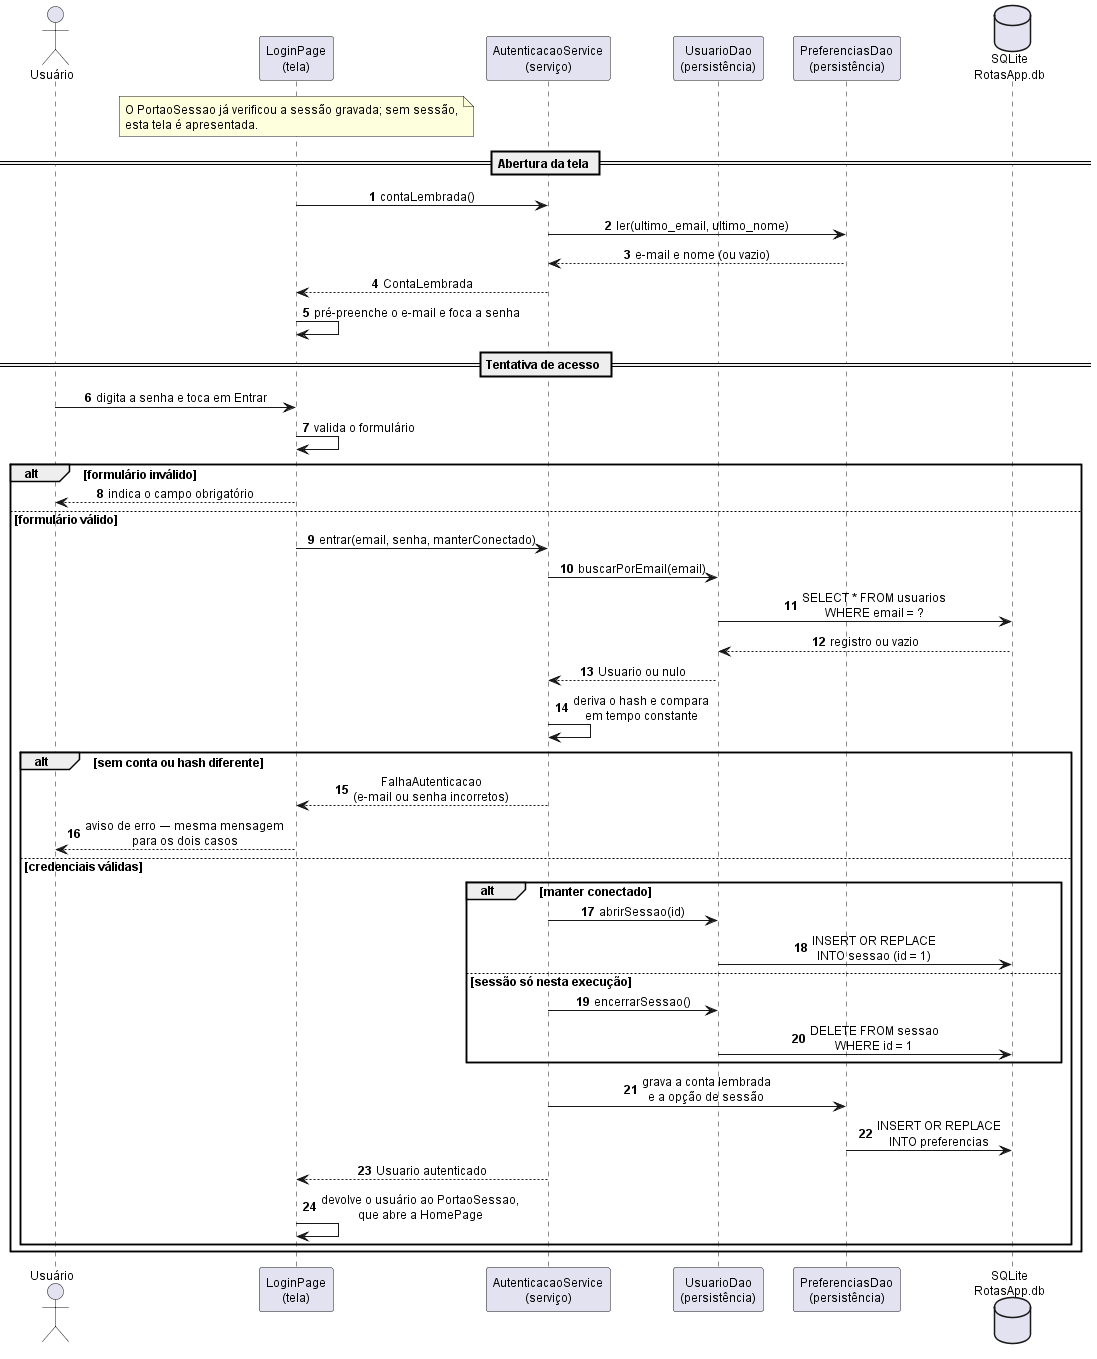
\includegraphics[width=1\linewidth]{imagens/sequencia-autenticacao.png}
    \vspace{2pt}
    \footnotesize Fonte: o próprio autor (2026)
\end{figure}

\subsection{Navegação assistida}

A navegação assistida acompanha a posição do veículo durante a execução da rota. A tela mantém em destaque o próximo ponto da ordem de visita, informa a distância e o sentido até ele e apresenta o trajeto completo sobre o mapa, com a posição atual do veículo em sobreposição às paradas.

O avanço entre paradas é automático: quando o veículo entra em um raio de cinquenta metros do ponto-alvo, o sistema passa a apontar para a parada seguinte e comunica a chegada. Esse raio foi adotado por ser compatível com a precisão do sinal de GPS em área urbana e com a extensão de um quarteirão, evitando exigir que o motorista pare exatamente sobre a coordenada. Como a precisão do sinal pode ser insuficiente em determinados trechos, a tela também permite avançar manualmente para a próxima parada.

Registra-se, com clareza, que se trata de uma navegação assistida e não de uma navegação curva a curva: o sistema não recalcula o trajeto a cada desvio da malha viária nem emite comandos de voz. O que a funcionalidade resolve é o problema identificado no levantamento de requisitos, que é manter o motorista informado sobre qual é a próxima entrega e quanto falta para alcançá-la, aproveitando a ordem de visita já otimizada e o traçado previamente gravado.

\section{Ordenação das paradas}

A ordem de visita dos pontos é definida pelo \texttt{OtimizadorRotaService}. Determinar a menor rota que visita um conjunto de pontos e retorna ao início corresponde ao problema do caixeiro-viajante, cuja solução exata é inviável para instâncias de tamanho realista, pois o número de ordens possíveis cresce de forma fatorial. A estratégia adotada é, portanto, heurística e opera em duas etapas.

A primeira etapa é construtiva e emprega a heurística do vizinho mais próximo: partindo do ponto de origem, escolhe-se sempre o ponto ainda não visitado mais próximo do atual. O procedimento tem custo quadrático no número de pontos e produz rapidamente uma solução válida, mas tende a deixar um trecho longo para o final, pois as escolhas locais não consideram o fechamento do percurso.

A segunda etapa refina a solução por meio do método 2-opt: procura-se um par de arestas cuja troca encurte o percurso e, quando esse par é encontrado, o trecho entre elas é invertido. O procedimento se repete até que nenhuma inversão produza ganho. Nas rotas em circuito, o percurso é tratado como um ciclo cujo ponto de partida permanece fixo; nas rotas ponto a ponto, tanto o ponto de partida quanto o de chegada são preservados, pois representam a escolha explícita do usuário. O número de inversões aplicadas e a redução obtida são registrados e apresentados ao usuário, o que torna o efeito do refinamento verificável na própria interface.

O fluxo completo do algoritmo é apresentado na Figura \ref{fig:atividades-otimizacao}. O diagrama mostra a validação de entrada, a fixação dos pontos que não podem mudar de posição, as duas etapas de construção e refinamento com os seus laços de repetição e as condições de parada, além do resultado devolvido ao repositório. Os pontos de decisão correspondem exatamente às guardas implementadas no serviço: a exigência de ao menos dois pontos com coordenadas, o critério de ganho do 2-opt e o limite de passagens que evita laços longos.

\begin{figure}[!ht]
    \centering
    \caption{Fluxo do algoritmo de ordenação das paradas}
    \label{fig:atividades-otimizacao}
    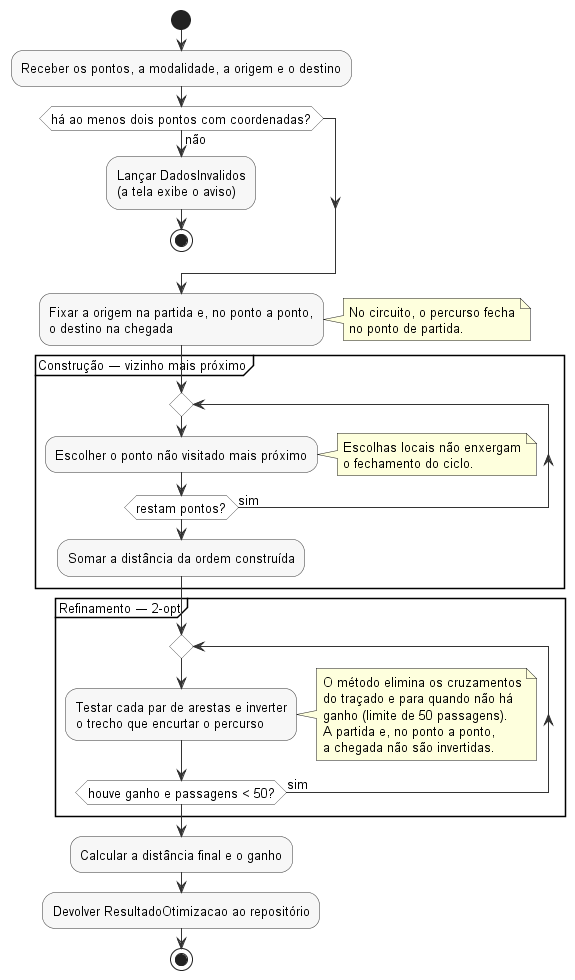
\includegraphics[width=1\linewidth]{imagens/atividades-otimizacao.png}
    \vspace{2pt}
    \footnotesize Fonte: o próprio autor (2026)
\end{figure}

A qualidade do resultado é verificada por teste automatizado que compara a distância obtida pela heurística com a menor distância possível, calculada por força bruta sobre todas as ordens de visita de uma instância pequena. O teste exige que a solução heurística não seja inferior ao ótimo, o que seria impossível, e que não exceda o ótimo em mais de quinze por cento.

\section{Tratamento de falhas e degradação controlada}

Os requisitos de confiabilidade preveem tolerância a falhas de rede e recuperação da rota \cite{sriVisao2025}. A implementação atende a esse requisito por meio de três mecanismos.

O primeiro é o recuo para o cálculo local. Quando o serviço de roteamento não responde, o trajeto é estimado em linha reta a partir das coordenadas, com a duração calculada pela velocidade urbana média assumida de trinta quilômetros por hora. A origem do cálculo é gravada junto com a rota e informada na interface, de modo que o usuário saiba que o traçado apresentado não segue as vias reais e possa recalcular o trajeto quando houver conexão.

O segundo é o limite de tempo das requisições externas. O serviço de roteamento é consultado com limite de vinte segundos, valor deliberadamente inferior aos trinta segundos estabelecidos como requisito de desempenho \cite{sriEspecComp2025}, para que mesmo o pior caso, que é o recuo para a estimativa local, permaneça dentro do prazo aceitável.

O terceiro é o controle de uso do serviço de geocodificação. A política de uso do Nominatim recomenda no máximo uma requisição por segundo por aplicação. O serviço implementado impõe um intervalo mínimo entre consultas externas e mantém um cache local dos endereços já convertidos, de modo que a repetição de um mesmo endereço não gera tráfego e o formulário responde de imediato.

As falhas são traduzidas, nos serviços, para exceções de domínio que já carregam uma mensagem em português adequada ao usuário, enquanto o detalhe técnico é preservado para depuração. Nenhuma tela exibe ao usuário o texto cru de um erro de rede ou de banco de dados.

\section{Verificação por análise estática e testes automatizados}

A verificação do código foi conduzida em dois níveis automatizados. O primeiro é a análise estática, executada pela ferramenta de análise do ambiente Flutter com as regras do conjunto \texttt{flutter\_lints}: a versão consolidada do código não apresenta nenhum aviso nem erro. Essa análise cobre erros de tipagem, uso incorreto de contexto de interface após operações assíncronas, importações não utilizadas e demais más práticas verificáveis sem execução.

O segundo nível é a suíte de testes automatizados, composta por cento e oito testes distribuídos em seis arquivos, conforme a Tabela \ref{tab:testes}. Os testes de persistência e de autenticação executam contra um banco SQLite em memória criado com o mesmo esquema e as mesmas migrações utilizados em produção, o que garante que a verificação incida sobre o esquema real e não sobre uma cópia que poderia divergir. As chamadas aos serviços externos são substituídas por respostas simuladas, de modo que os testes não dependem de rede e são determinísticos.

\begin{table}[!ht]
    \centering
    \caption{Distribuição dos testes automatizados}
    \label{tab:testes}
    \begin{tabular}{p{5cm}p{2cm}p{8cm}}
        \hline
        \textbf{Arquivo} & \textbf{Testes} & \textbf{O que verifica} \\
        \hline
        geo\_utils\_test.dart & 20 & Distâncias pela fórmula de Haversine contra valores conhecidos, formatação de distância e duração, leitura e gravação da geometria e tolerância a registros corrompidos \\
        otimizador\_rota\_test.dart & 9 & Corretude do refinamento 2-opt em ordens cruzadas, preservação dos pontos de partida e chegada, descarte de pontos sem coordenadas e proximidade do ótimo obtido por força bruta \\
        navegacao\_test.dart & 16 & Avanço entre paradas pelo raio de chegada, instrução apresentada, distância restante em rotas abertas e em circuitos e cálculo do progresso \\
        autenticacao\_test.dart & 25 & Derivação e comparação de senha, validações de cadastro, vínculo dos pontos legados, troca de senha, exclusão de conta, identidade das mensagens de erro, conta lembrada e política de sessão \\
        persistencia\_test.dart & 30 & Criação do esquema, migração da versão 1 preservando os dados, operações de cada objeto de acesso a dados, preferências, integridade referencial, transação de gravação de rota, cache e limites de uso da geocodificação e recuo do roteamento \\
        widget\_test.dart & 8 & Validação do formulário de acesso, fluxo completo de criação de conta até a tela inicial e acesso com conta lembrada, todos com banco em memória \\
        \hline
        \textbf{Total} & \textbf{108} & \\
        \hline
    \end{tabular}
    \vspace{2pt}
    \footnotesize Fonte: o próprio autor (2026)
\end{table}

Além desses dois níveis, a compilação completa do aplicativo foi executada com sucesso para dois alvos distintos: o alvo web, que confirma que o conjunto do código-fonte compila de ponta a ponta, e o alvo Android, cujo pacote de instalação foi gerado sem falhas. A geração do pacote Android constituiu a verificação mais exigente, porque envolve, além da compilação do código Dart, a compilação do código nativo, a validação do manifesto de permissões e a vinculação das bibliotecas de plataforma usadas pelo acesso ao banco de dados e à localização.

Sobre essa base, a execução funcional foi verificada em emulador Android, com o aplicativo instalado e operado nos fluxos descritos na especificação de caso de uso. A verificação cobriu a criação de conta e a abertura de sessão, o cadastro de pontos, a conversão de endereços em coordenadas pelo serviço Nominatim, a renderização do mapa com os blocos cartográficos e o marcador do ponto, a geração de uma rota em circuito com quatro paradas, a gravação e a reabertura da rota salva e a navegação assistida, incluindo a solicitação e a concessão da permissão de localização e o avanço automático entre paradas. Nessa execução o cálculo da rota foi efetivamente resolvido pelo serviço de roteamento, e não pelo recuo local: o resultado registrado foi de 23,9 quilômetros, 40 minutos de duração estimada e traçado sobre as vias reais de Londrina, o que confirma a integração com o serviço externo.

Um comportamento observado nessa execução merece registro, por validar a estratégia de migração descrita na seção anterior. Ao instalar a versão consolidada sobre um banco criado pela primeira versão do aplicativo, os pontos então existentes, que não possuíam proprietário, foram vinculados à primeira conta criada no dispositivo e passaram a aparecer na lista do usuário, em vez de ficarem órfãos ou inacessíveis. A migração, portanto, foi exercitada sobre dados reais e não apenas sobre um banco de teste.

A política de sessão também foi verificada nos dois sentidos. Com a opção de manter conectado marcada, o aplicativo foi encerrado e reaberto e apresentou diretamente a lista de pontos, sem passar pela tela de acesso. Com a opção desmarcada, o encerramento e a reabertura devolveram a tela de acesso, porém com a conta já identificada e apenas o campo de senha a preencher — ou seja, o atrito fica restrito à digitação da senha, e não à identificação da conta.

Cabe registrar o que permanece pendente. A execução em emulador não reproduz as condições de campo: a variação real da precisão do sinal de GPS, o comportamento em conectividade intermitente e o consumo de energia só podem ser avaliados em aparelho físico, em uso prolongado. Além disso, as métricas de tempo de resposta e de assertividade declaradas nos requisitos dependem de medição sistemática em campo e da validação das rotas junto ao usuário, o que está previsto como continuidade do trabalho.

\section{Interface do aplicativo}

As telas da versão consolidada são apresentadas nas Figuras \ref{fig:tela-login} a \ref{fig:tela-navegacao}. Todas as capturas foram obtidas do aplicativo em execução no emulador, com dados de demonstração cadastrados, e não de protótipos.

A Figura \ref{fig:tela-login} apresenta a tela de acesso. O aplicativo abre nessa tela sempre que não há sessão ativa, o que materializa o requisito de autenticação obrigatória: não existe caminho de acesso às funcionalidades sem a identificação do usuário. A conta do último acesso aparece identificada no topo, de modo que resta ao usuário digitar apenas a senha, e a opção de manter a sessão entre execuções vem marcada por padrão.

\begin{figure}[!ht]
    \centering
    \caption{Tela de acesso ao sistema}
    \label{fig:tela-login}
    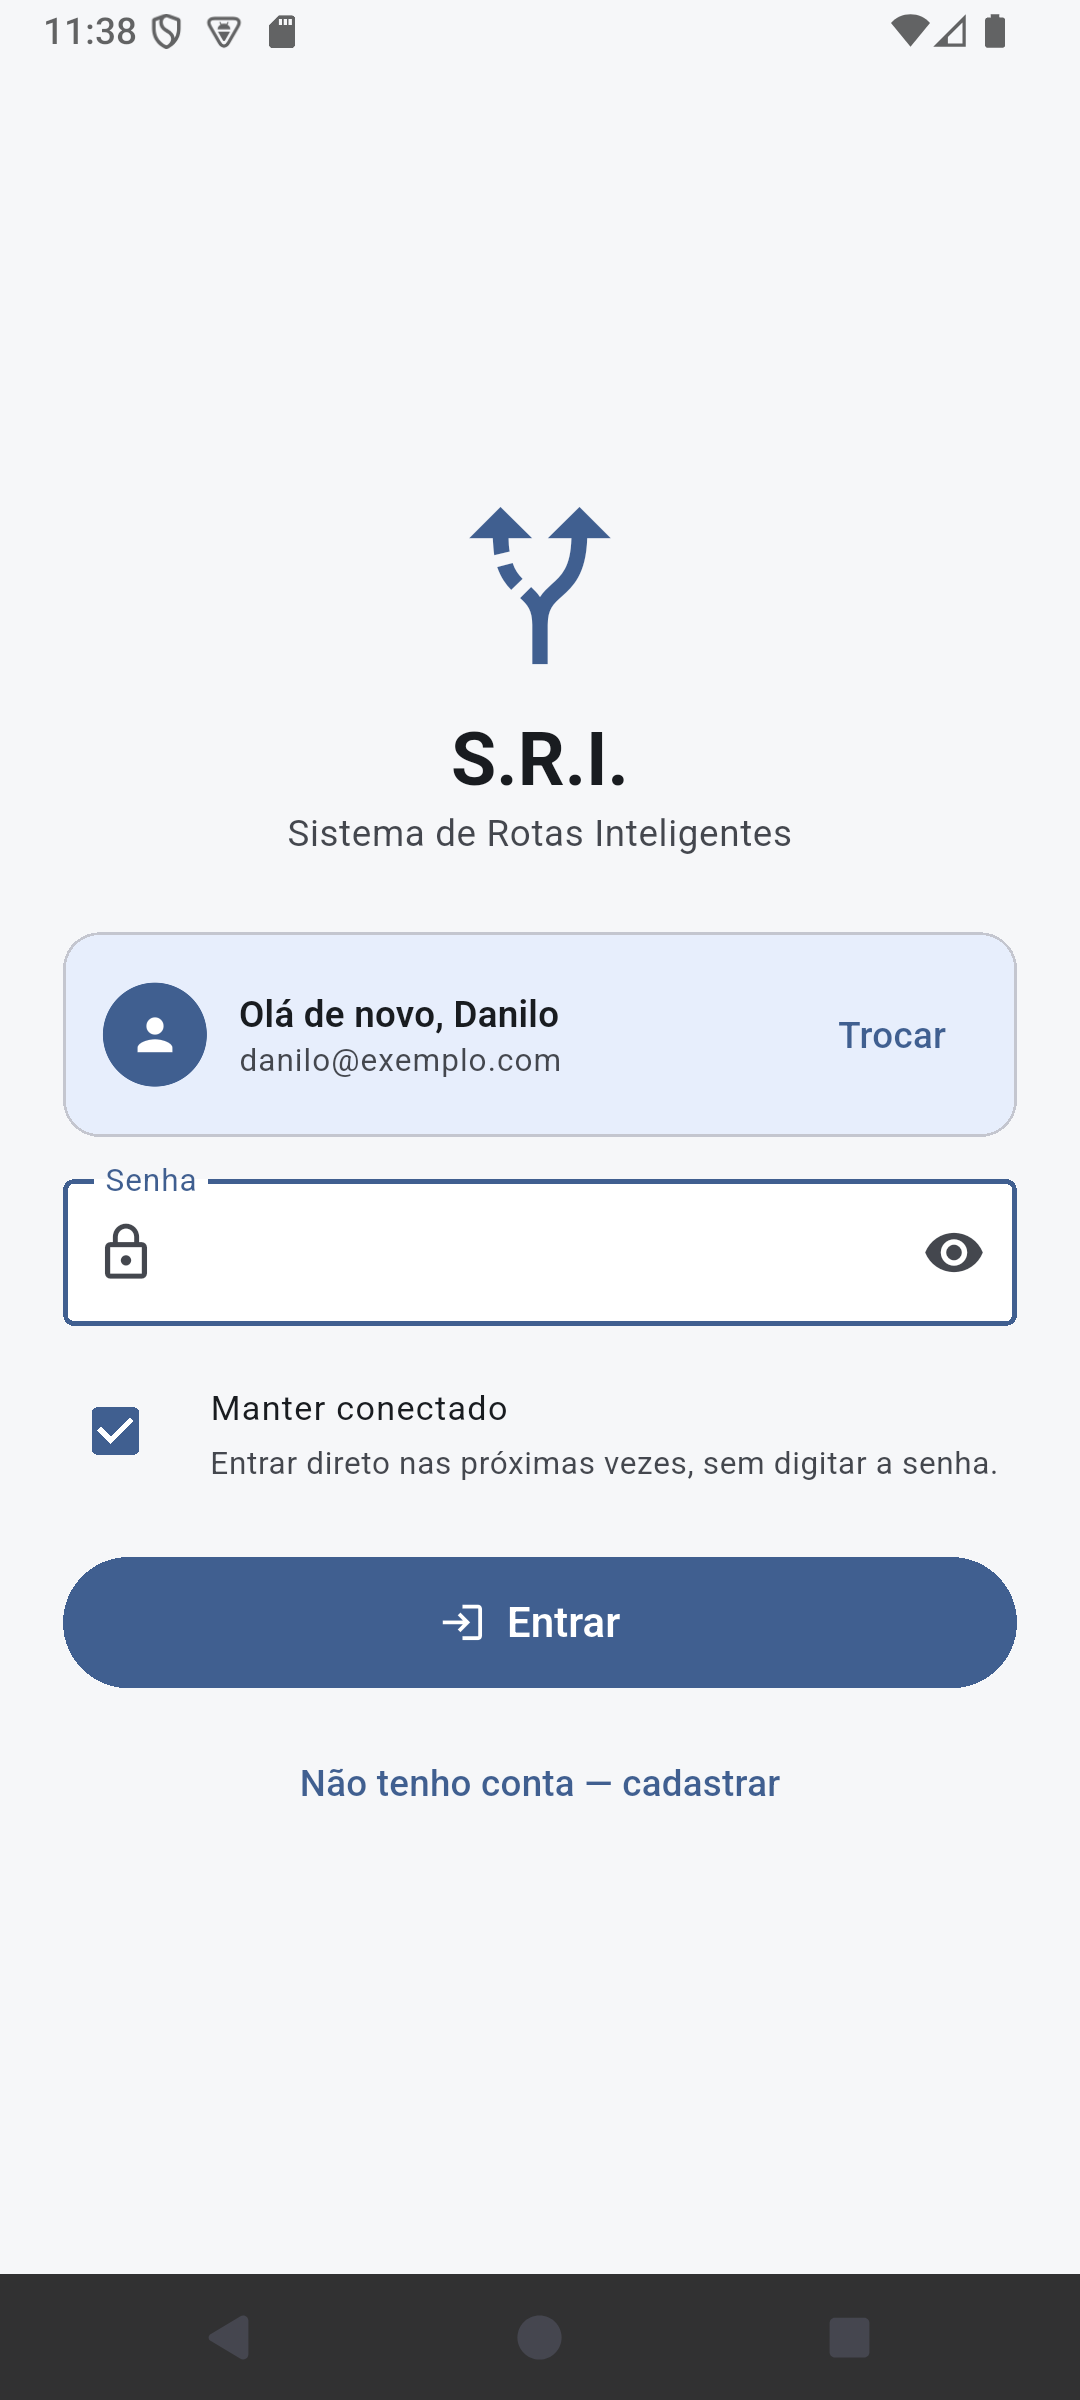
\includegraphics[width=0.5\linewidth]{imagens/tela-login.png}
    \vspace{2pt}
    \footnotesize Fonte: captura do aplicativo em execução (2026)
\end{figure}

A Figura \ref{fig:tela-pontos} apresenta a lista de pontos cadastrados, com o nome, o endereço e as ações de editar e excluir, além do indicador de que o endereço já foi localizado no mapa. O acesso ao mapa de cada ponto se dá pelo toque sobre o item da lista.

\begin{figure}[!ht]
    \centering
    \caption{Tela de pontos cadastrados}
    \label{fig:tela-pontos}
    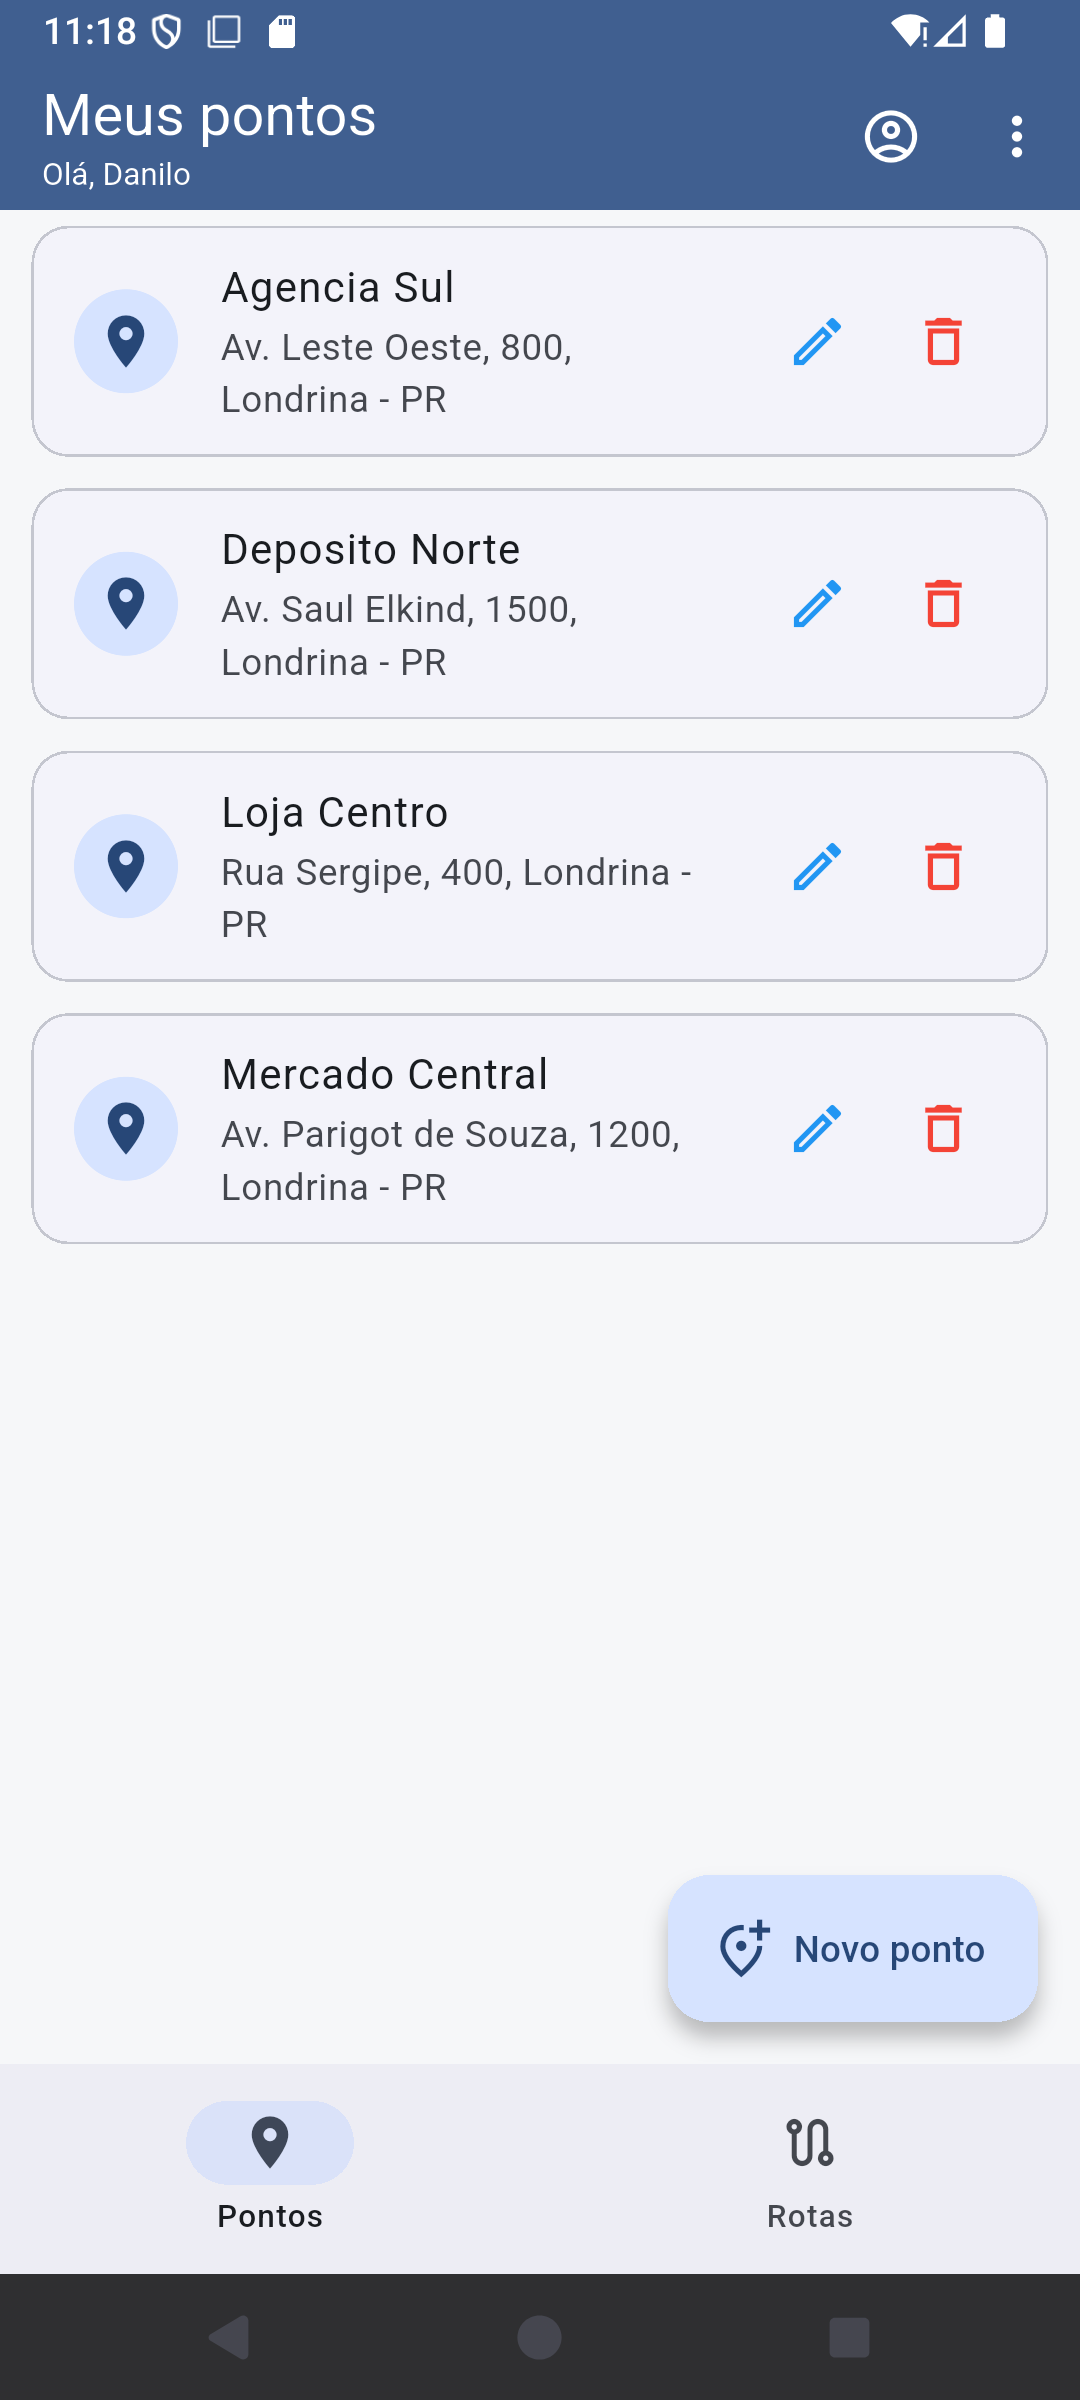
\includegraphics[width=0.5\linewidth]{imagens/tela-pontos.png}
    \vspace{2pt}
    \footnotesize Fonte: captura do aplicativo em execução (2026)
\end{figure}

A Figura \ref{fig:tela-previa-rota} apresenta o resultado do cálculo de uma rota em circuito com quatro paradas. A tela reúne o traçado sobre o mapa, as métricas do percurso, o modo de operação, a origem efetiva do cálculo e a ordem de visita otimizada, com a indicação da partida, das paradas intermediárias e do retorno que fecha o circuito.

\begin{figure}[!ht]
    \centering
    \caption{Prévia de rota em circuito calculada}
    \label{fig:tela-previa-rota}
    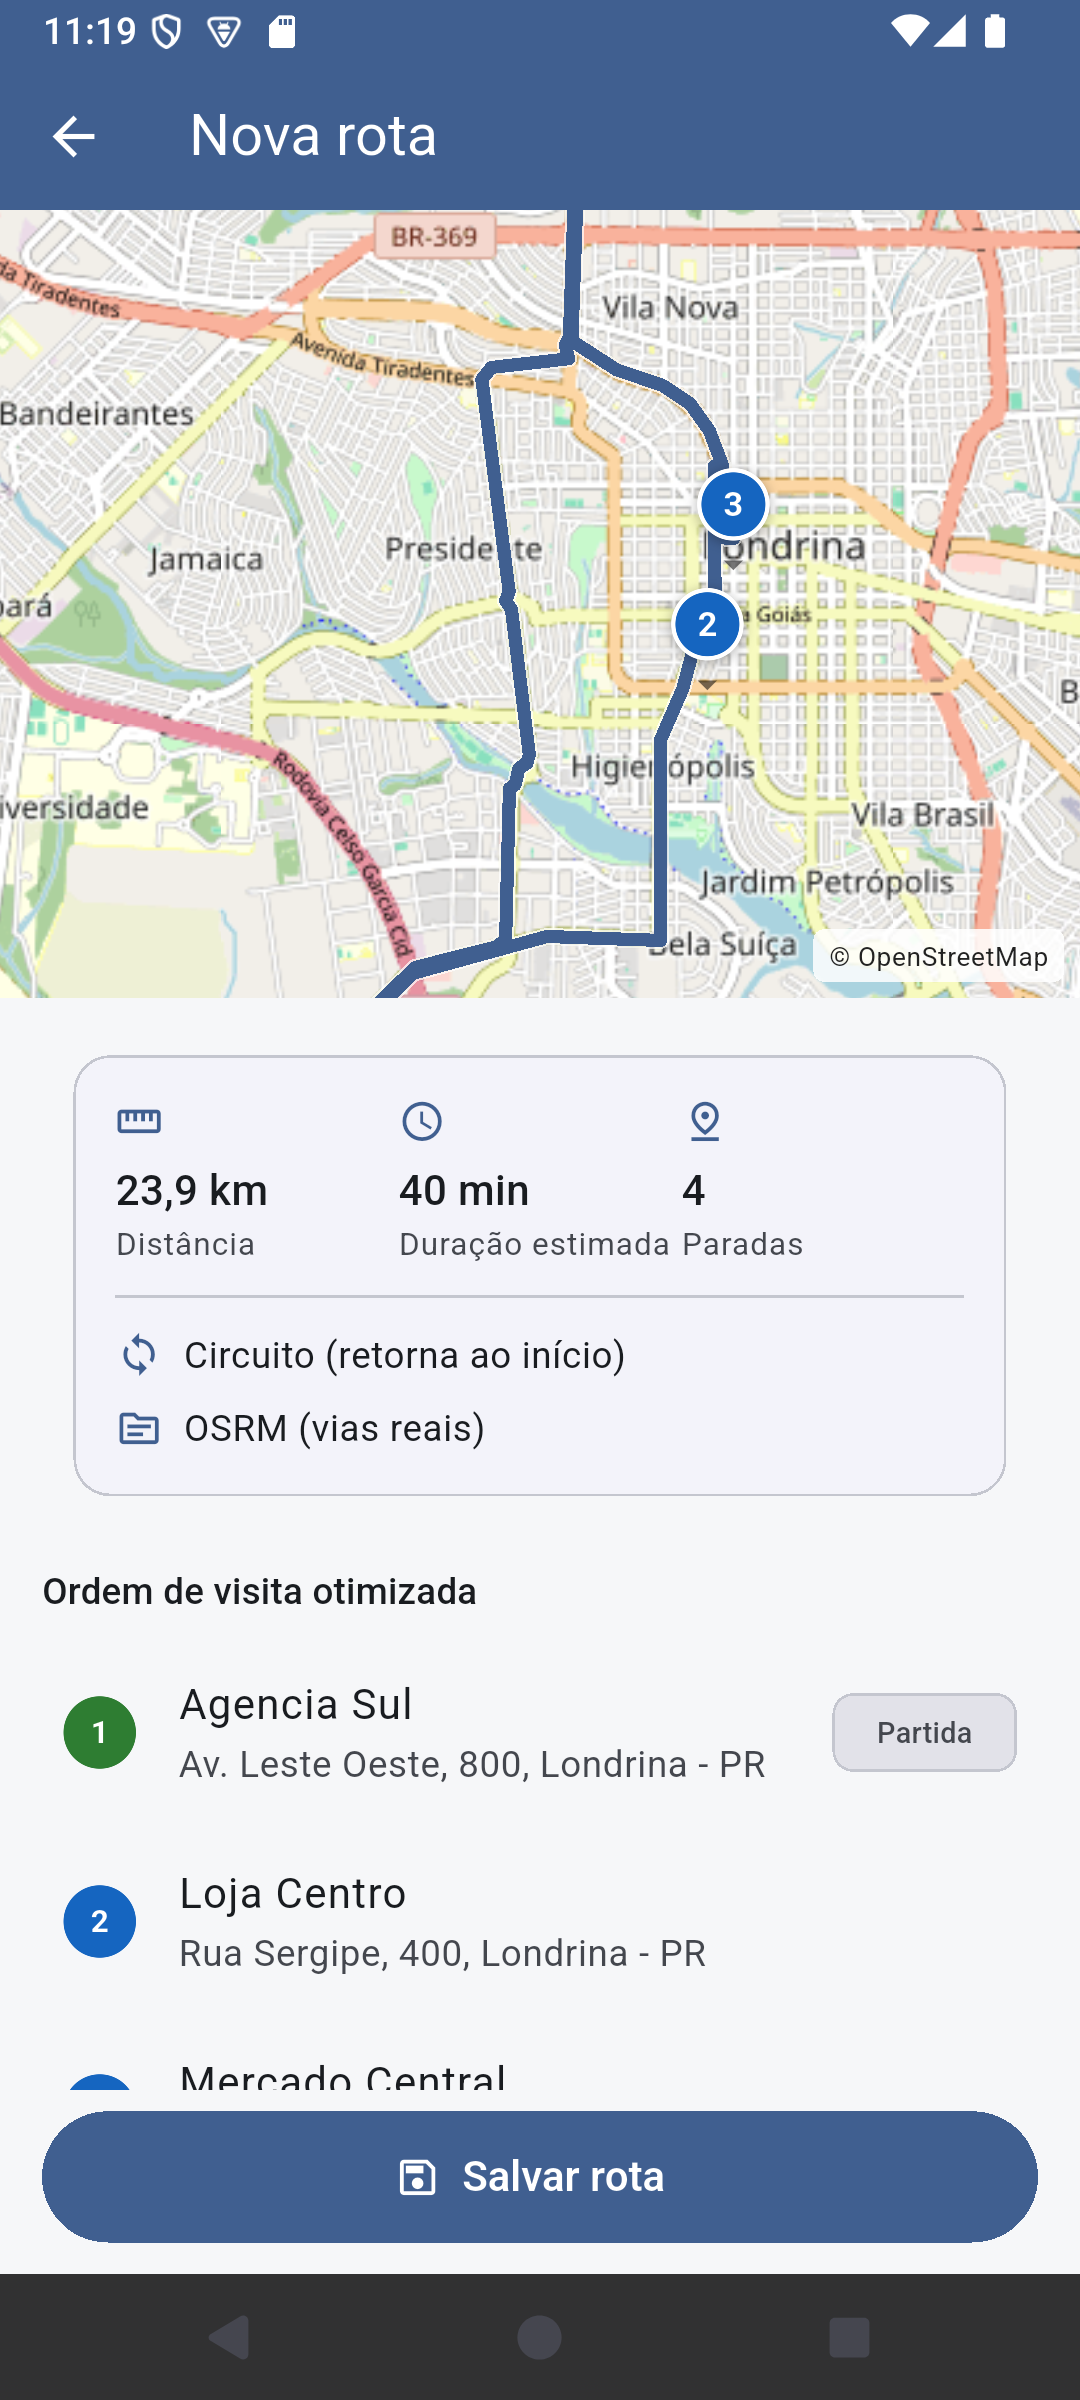
\includegraphics[width=0.5\linewidth]{imagens/tela-previa-rota.png}
    \vspace{2pt}
    \footnotesize Fonte: captura do aplicativo em execução (2026)
\end{figure}

A Figura \ref{fig:tela-rotas-salvas} apresenta a lista de rotas salvas, com a modalidade, a quantidade de paradas, a distância e a duração de cada trajeto, além das ações de edição e de exclusão.

\begin{figure}[!ht]
    \centering
    \caption{Tela de rotas salvas}
    \label{fig:tela-rotas-salvas}
    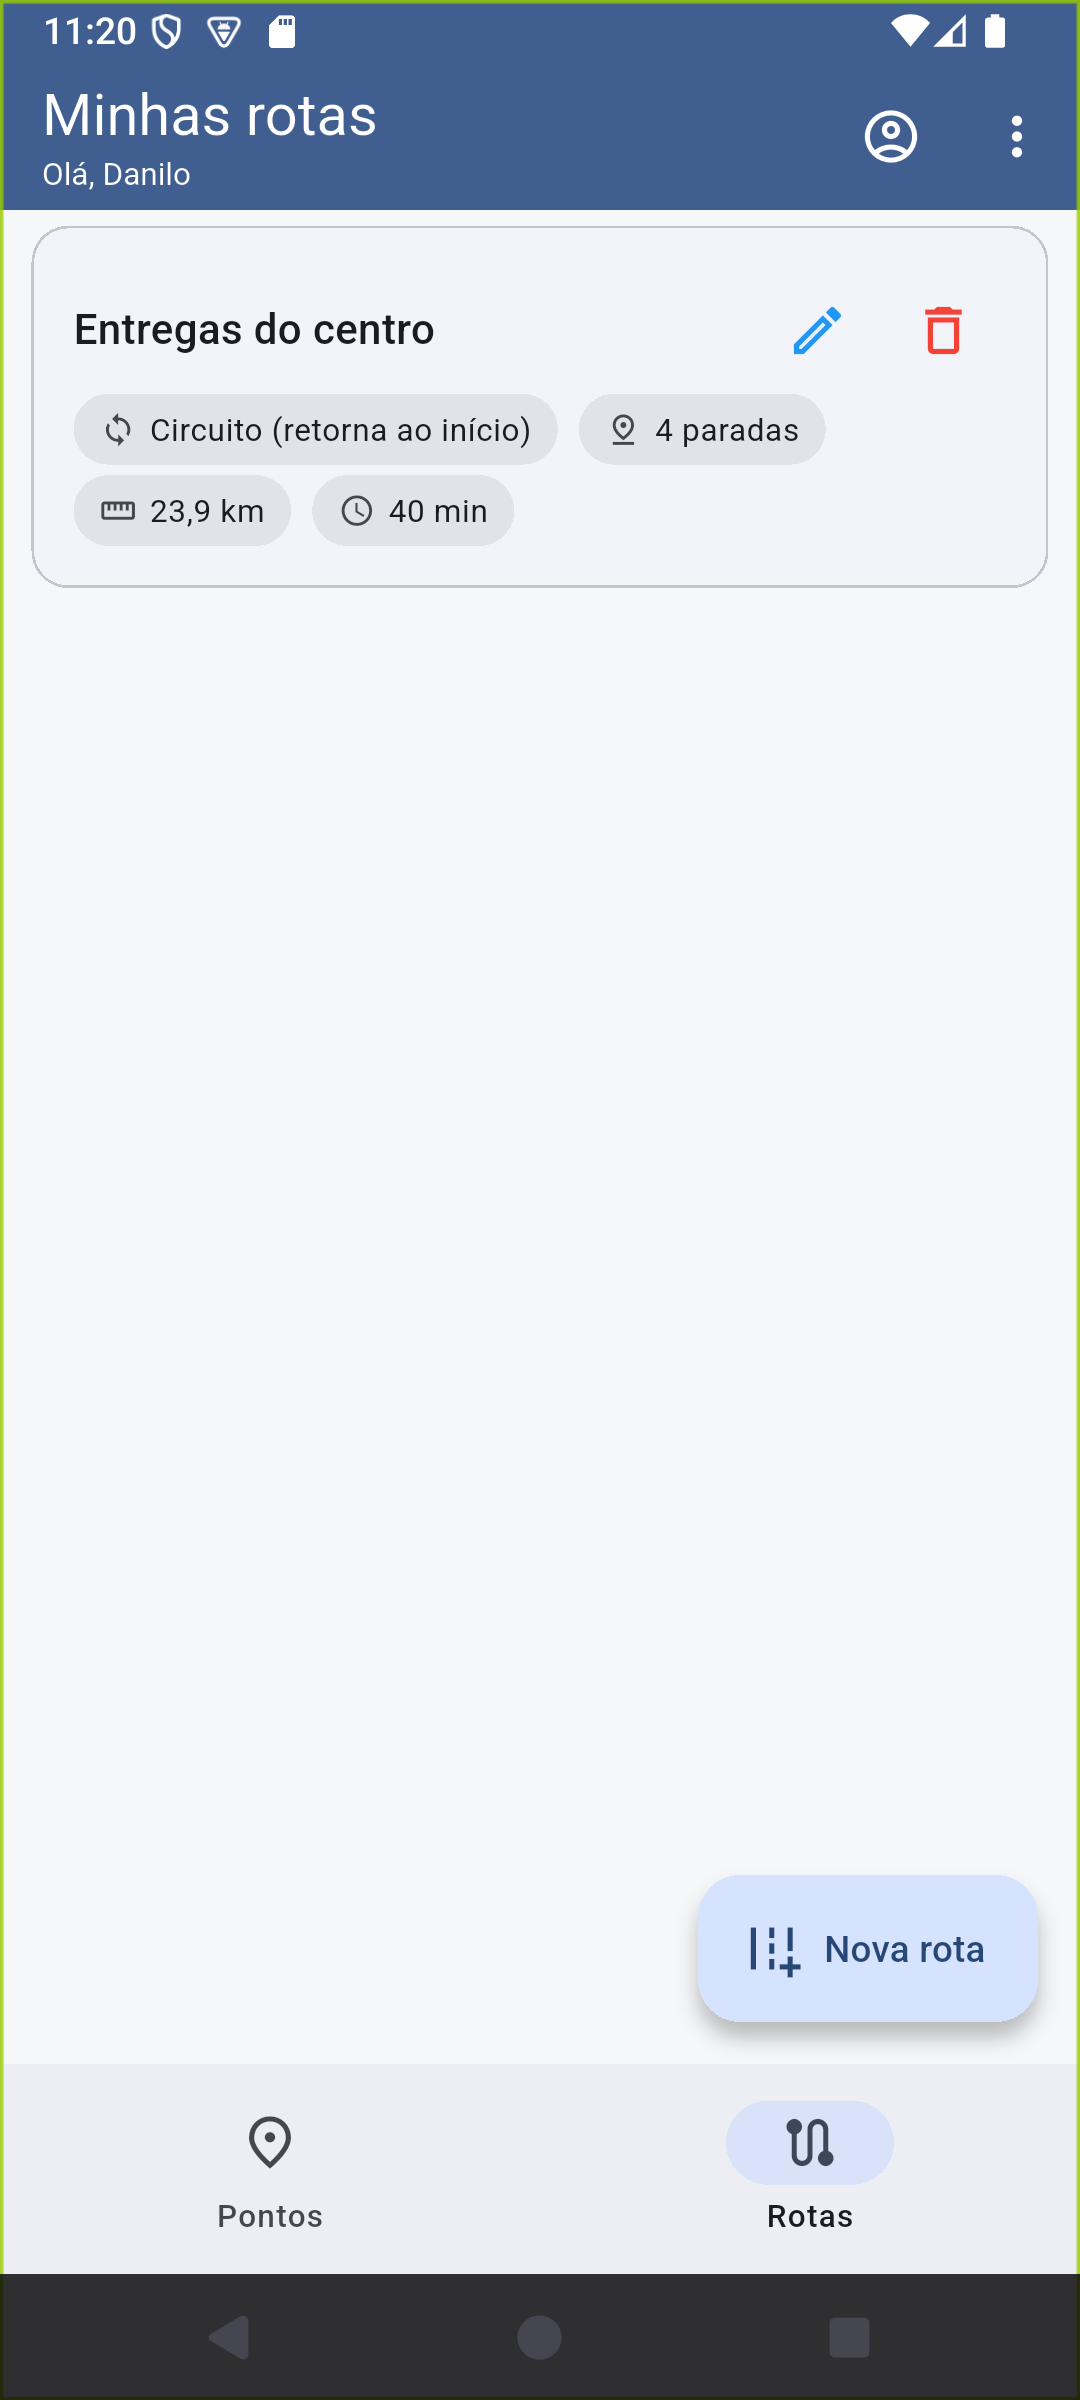
\includegraphics[width=0.5\linewidth]{imagens/tela-rotas-salvas.png}
    \vspace{2pt}
    \footnotesize Fonte: captura do aplicativo em execução (2026)
\end{figure}

A Figura \ref{fig:tela-navegacao} apresenta a navegação assistida em curso. A faixa superior traz a instrução do próximo ponto, com a distância e o sentido; o mapa exibe o traçado e a posição atual do veículo; e o painel inferior informa a parada em curso, a distância restante, o progresso do percurso e as ações de centralizar o mapa e de avançar manualmente para a próxima parada.

\begin{figure}[!ht]
    \centering
    \caption{Tela de navegação assistida}
    \label{fig:tela-navegacao}
    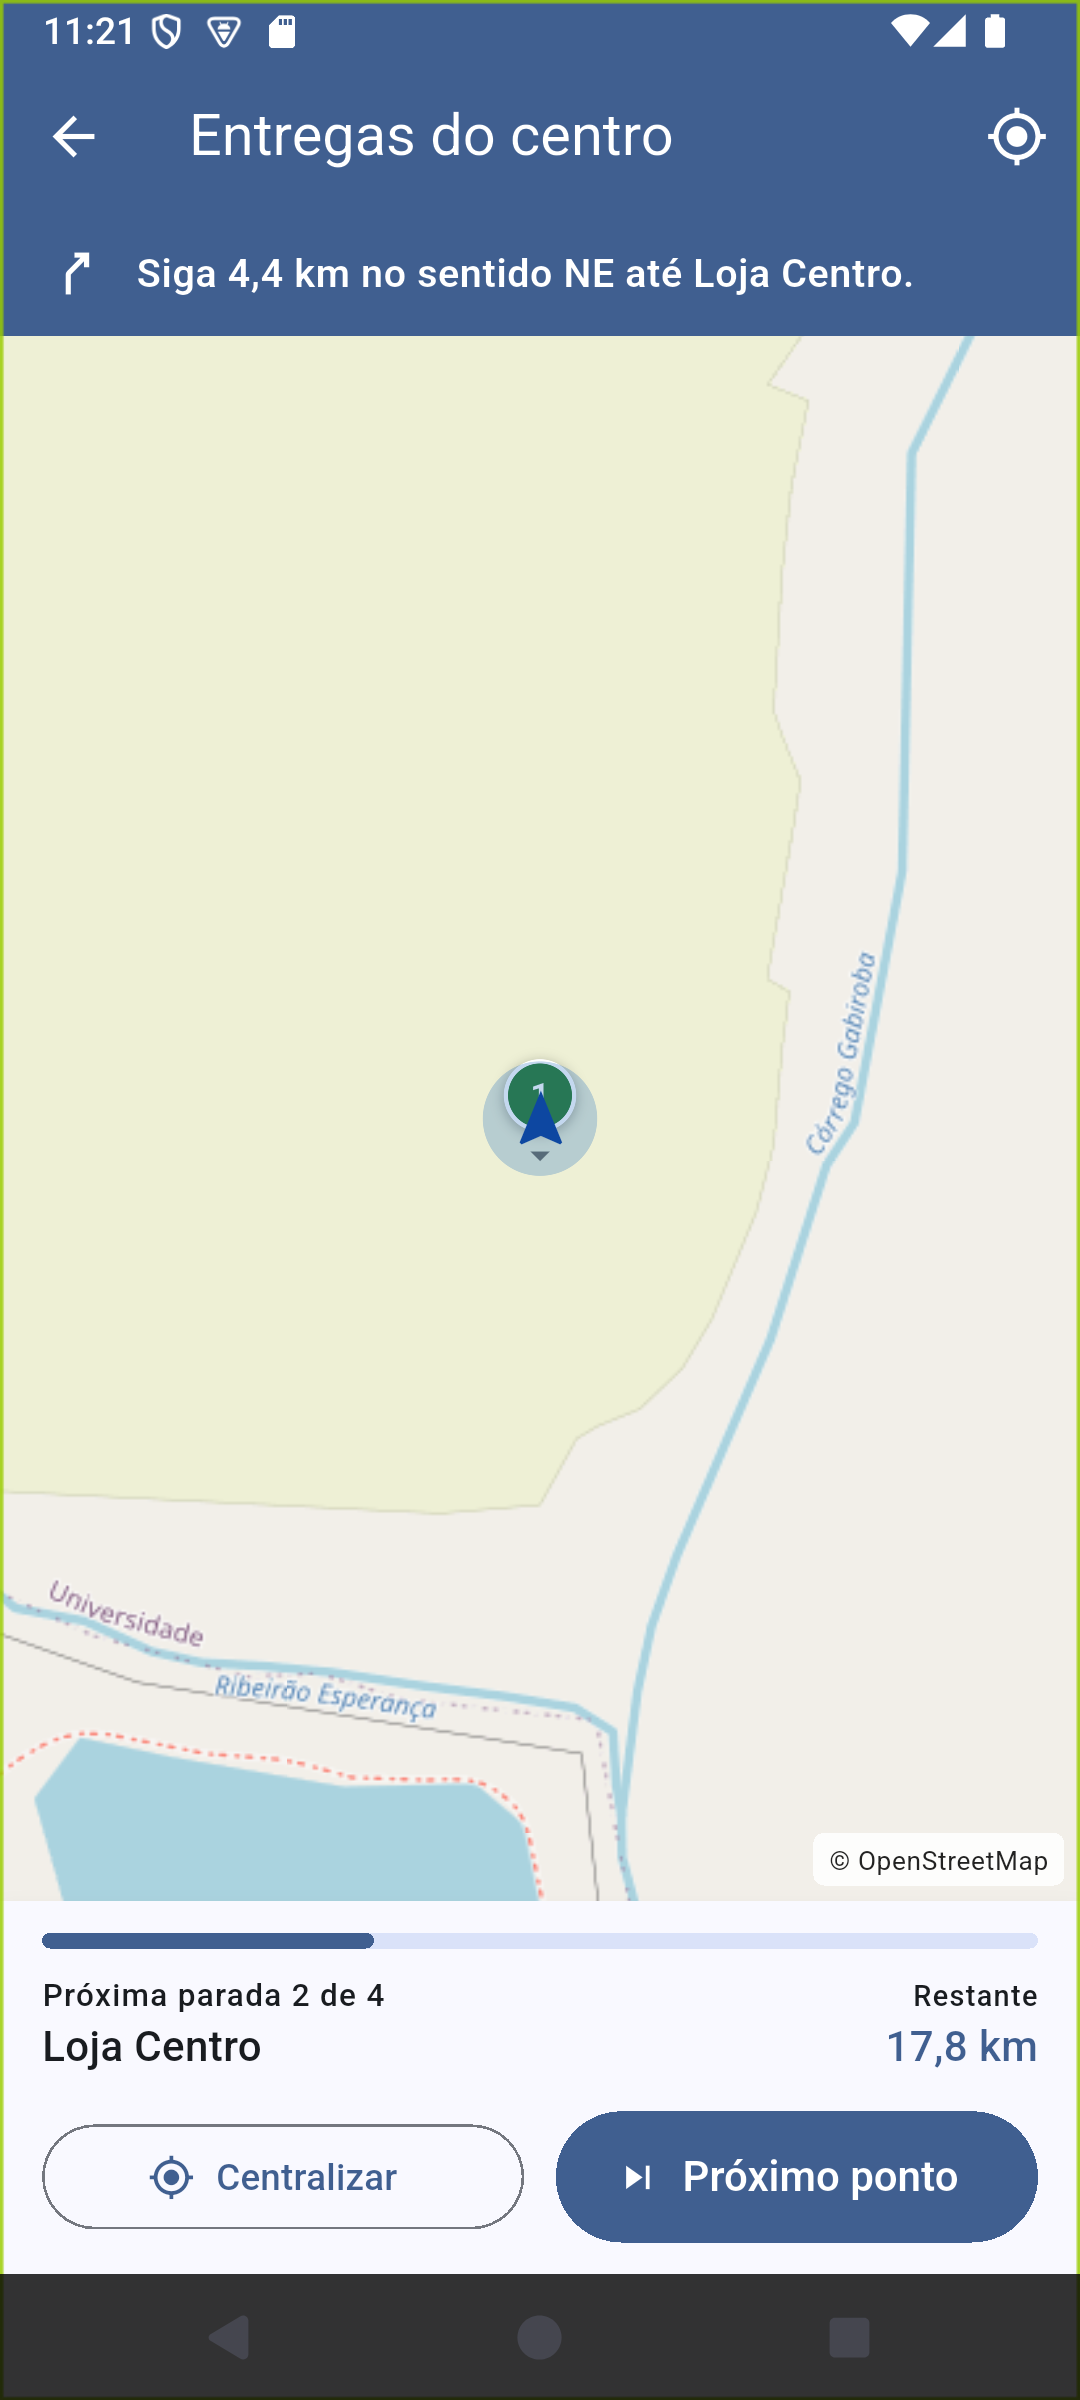
\includegraphics[width=0.5\linewidth]{imagens/tela-navegacao.png}
    \vspace{2pt}
    \footnotesize Fonte: captura do aplicativo em execução (2026)
\end{figure}

\section{Métricas do código-fonte}

A Tabela \ref{tab:metricas-codigo} apresenta o tamanho da versão consolidada, por camada. Os números incluem as linhas de comentários e de documentação das classes, que foram mantidas como parte do artefato entregue.

\begin{table}[!ht]
    \centering
    \caption{Tamanho do código-fonte por camada}
    \label{tab:metricas-codigo}
    \begin{tabular}{p{15cm}rr}
        \hline
        \textbf{Camada} & \textbf{Arquivos} & \textbf{Linhas} \\
        \hline
        Apresentação (telas) & 11 & 2.729 \\
        Serviços & 6 & 1.271 \\
        Persistência (objetos de acesso e banco) & 8 & 950 \\
        Componentes visuais reutilizáveis & 4 & 610 \\
        Infraestrutura (tema, exceções, utilitários e montagem) & 4 & 359 \\
        Modelo de domínio & 3 & 351 \\
        Ponto de entrada e portão de sessão & 2 & 126 \\
        \hline
        \textbf{Total do aplicativo} & \textbf{38} & \textbf{6.396} \\
        \hline
        Testes automatizados & 7 & 1.916 \\
        \hline
    \end{tabular}
    \vspace{2pt}
    \footnotesize Fonte: o próprio autor (2026)
\end{table}
